\section{Theory and Procedure}
\label{sec:theory}
% In this section we describe the theory and procedures used to arrive 
% at a function and its implementation for the unknown component. We
% also show how to explore the solution space for implementable functions. 

% %\subsection{Reference specification is polynomial f}
% Consider a specification polynomial $f$ and a gate-level circuit $C$
% that implements $f$. Model the circuit by way of polynomials $F =
% \{f_1,\dots,f_s\}\in \mathbb{F}_q[x_1,\dots, x_n]$, where
% variables $x_1,\dots,x_n$ denote the nets in the circuit. The set $F$
% generates an ideal $J=\langle F \rangle$, and let $J_0=\langle
% x_l^q-x_l: 1\leq l\leq n\rangle$ be the set of all vanishing polynomials.

% As described in \cite{lv:tcad2013}, the equivalence check between $f$
% and $C$ can be formulated as an ideal membership test that checks if
% $f \in J + J_0$. Thus, one can compute a \Grobner basis
% $G=GB(J+J_0) = \{g_1,\dots,g_t\}$, and check if $f
% \xrightarrow{G}_+0$? If the circuit $C$ indeed implements $f$, 
% $f \xrightarrow{G}_+ 0$ and $f$ can be written as a linear combination
% of $g_1\dots,g_t$, and also of $f_1\dots, f_s$, by virtue of
% Eqns. (\ref{eqn:matrix}),(\ref{eqn:imt}), and (\ref{eqn:imt_orig}).

% The \Grobner basis algorithm has very high exponential complexity
% ($q^{O(n)}$ in our case). In \cite{lv:tcad2013}, it was further shown
% that this complexity can be overcome by deriving a specialized term
% order by analyzing the topology of the given circuit. It relies on the
% condition that {\it when the leading terms of all polynomials in a
% generating set $F=\{f_1,\dots,f_s\}$ are relatively prime, then $F$
% already constitutes a GB, i.e. $F = GB(F)$}. We restate the result:


% \begin{Proposition} \label{prop:top-order}
% (From \cite{lv:tcad2013}) Let $C$ be any arbitrary combinational
%   circuit. Let $\{x_1, \dots, x_n\}$ denote the set of all variables
%   (signals) in $C$. Starting from the primary outputs, perform
%   a {\it reverse topological traversal} of the circuit and order the
%   variables such that $x_i > x_j$ if $x_i$ appears earlier in the
%   reverse topological order. Impose a {\it lex} term order $>$ to
%   represent each gate as a polynomial $f_i$, s.t. $f_i = x_i +
%   tail(f_i)$. Then the set of all polynomials  $\{f_1, \dots, f_s\}$
%   forms a Gr\"obner basis G, as $lt(f_i)=x_i$ and $lt(f_j)=x_j$ for 
%   $i\neq j$ are relatively prime. This term order $>$ is called the 
%   {\bf Reverse Topological Term Order (RTTO)}.
% \end{Proposition}

% Imposition of RTTO $>$ on the polynomials of the circuit has the
% effect of making every gate output variable $x_i$ a leading term of
% $f_i$. Since every gate output is unique, $lm(f_i)=x_i,$ $lm(f_j)=x_j
% :\forall i\neq j$ the leading terms become relatively prime. As a result, the set $F$ 
% already constitutes a GB ($G=F$). Moreover, it was further shown in
% \cite{lv:tcad2013} that under RTTO, the set $F \cup F_0$ forms the
% \Grobner basis of $J + J_0$. As a result, the verification test
% can be carried out simply by the division of $f$ modulo the \Grobner
% basis $F\cup F_0$ and checking if the remainder is 0; i.e. $f
% \xrightarrow{F,F_0}_+r$, and checking if $r = 0$? When $C$ does
% implement $f$, $r=0$ and $f = u_1f_1+\dots+u_sf_s + \sum_{i=1}^n
% H_i\cdot(x_i^q-x_i)$. 

% An important effect of RTTO $>$ is that each gate $\mathcal{G}_i$ is
% represented by a polynomial of the type $f_i = x_i +
% \text{tail}(f_i)$.  RTTO ensures that
% every variable $x_j$ that appears in $\text{tail}(f_i)$ satisfies
% $x_i>x_j$. These properties will be exploited in our technique. 

% \subsection{The unknown component}
% Now consider that verification has been performed between $f$ and $C$,
% and it is found that $C$ {\bf does not} implement $f$. Further, assume
% that post-verification debugging identifies the gate $\mathcal{G}_i
% \in C$, with output net $x_i$ where a correction can be synthesized and
% implemented to meet the specification. We consider the gate
% $\mathcal{G}_i$ as the unknown component and attempt to identify a
% function for $\mathcal{G}_i$. More precisely, {\it we have to compute
%   a polynomial $f_i = x_i + \text{tail}(f_i)$ that identifies a
%   function implementable at gate $\mathcal{G}_i$} such that the
% circuit $C$ conforms to the specification $f$. 

% \begin{algorithm}
% \caption{unknown component function}\label{pseudouc}
% \begin{algorithmic}[1]
% \Require {$f,\{f_1\dots,f_{i-1},f_i,f_{i+1},\dots f_s\},f_i=x_i+P(X)$}
% \Ensure {polynomial function for P(X)}
% \Procedure{$uc\_function$}{}
% \State $J_1=\{f_1\dots f_{i-1},lt(f_i)\},J_2=\{f_{i+1}\dots f_s\},P(X)=0$
% \State impose $RTTO >$ on the polynomials~\ref{prop:top-order}
% \State $h_i,r = multivar\_division(f,J_1)$
% \If{$h_i$ is \textbf{not} a constant:} 
% \State $J_p = h_i,J_2$
% \State $G=\{g_1,\dots,g_t\}=Grobner\_basis(J_p)$
% \State $V=[v_1\dots v_t]=$extnd\_ideal\_membrshp$(G,r)$ //$r=[v_1\dots v_t]\cdot[g_1\cdots g_t]^T$
% \State $M=[m_1\dots m_s]=$extnd\_ideal\_membrshp$(J_p,G)$ //$[g_1\cdots g_t]^T = M\cdot[h_i,f_{i+1}\cdots f_s]^T$(~\autoref{eqn:matrix})
% \For{$i$ from $1,...,size(G)$}
% \State $P(X) = P(X)+(V[1,i]\cdot M[1,i])$
% \EndFor
% \Else
% \State $h_{iin}=inverse(h_i)$
% \State $r_i=h_{iin}\cdot r$
% \State $P(X)=multivar\_division(r_i,J_2)$
% \EndIf
% \State \Return $P(X)$
% \EndProcedure
% \end{algorithmic}
% \end{algorithm}

% \begin{algorithm}
% \caption{unknown component function(improved)}\label{pseudoucimp}
% \begin{algorithmic}[1]
% \Require {$f,\{f_1\dots,f_{i-1},f_i,f_{i+1},\dots f_s\},f_i=x_i+P(X)$}
% \Ensure {polynomial function for P(X)}
% \Procedure{$uc\_function$}{}
% \State $J_1=\{f_1\dots f_{i-1},lt(f_i)\},J_2=\{f_{i+1}\dots f_s\},P(X)=0$
% \State impose $RTTO >$ on the polynomials~\ref{prop:top-order}
% \State $h_i,r = multivar\_division(f,J_1)$
% \If{$h_i$ is \textbf{not} a constant:} 
% \State $J_p = h_i,J_2$
% \State $l=multivar\_division(h_i,J_2)$
% \State $J_l = l,J_2$
% \State $V=[v_1\dots v_t]=$extnd\_ideal\_membrshp$(J_l,r)$ //$r=[v_1\dots v_t]\cdot[l,\cdots f_s]^T$
% \State $M=[m_1\dots m_s]=$extnd\_ideal\_membrshp$(J_p,J_l)$ //$[l,\cdots f_s]^T = M\cdot[h_i,f_{i+1}\cdots f_s]^T$(~\autoref{eqn:matrix})
% \For{$i$ from $1,...,size(J_l)$}
% \State $P(X) = P(X)+(V[1,i]\cdot M[1,i])$
% \EndFor
% \Else
% \State $h_{iin}=inverse(h_i)$
% \State $r_i=h_{iin}\cdot r$
% \State $P(X)=multivar\_division(r_i,J_2)$
% \EndIf
% \State \Return $P(X)$
% \EndProcedure
% \end{algorithmic}
% \end{algorithm}

% First, we address the problem of computing a polynomial
% $f_i$ of the form $f_i:x_i+P(X)$ as an implementation of
% $\mathcal{G}_i$, where $x_i$ is the output of the gate
% $\mathcal{G}_i$, $X \subset \{x_1,\dots,x_n\}$ is a subset of the nets
% in the circuit that lie in the fanin cone of the gate $\mathcal{G}_i$,
% and $P(X) = \text{tail}(f_i)$ is a polynomial in $X$-variables,
% with coefficients in $\Fq$. Subsequently, we address the problem of
% identifying $f_i:x_i+P(X_{im})$ as an implementation of
% $\mathcal{G}_i$ where  $X_{im} \subset \{x_1,\dots,x_n\}$ is a {\it
%   given} set of variables corresponding to the internal nets of the
% circuit. This case corresponds to resolving the unknown component with
% more topological constraints imposed on $P(X_{im})$ by the user; say,
% when the immediate inputs ($X_{im}$) of the unknown gate
% $\mathcal{G}_i$ are known.  {\it Note that here we assume that the
%   unknown component can indeed be composed of the given $X_{im}$
%   variables}. 


% As described above, for a correct implementation,
% $$f \in \langle f_1,..,f_s\rangle + \langle x_l^q-x_l: 1\le l \le n\rangle.$$

% We impose RTTO $>$ on the ring, which ensures that the set
% $\{f_1,\dots,f_s\}\cup \{x_1^q-x_1,\dots,x_n^q-x_n\}$ itself
% constitutes a \Grobner basis. Thus
% $f\xrightarrow{f_1,\dots,f_s,x_l^q-x_l}_+0$. Using Lemma
% \ref{lem:imt}, we can rewrite $f$ in terms of its generators as:   

% \begin{equation}\label{eqn1}
% f = h_1f_1 + h_2f_2 + \dots+h_if_i+\dots+h_sf_s + \sum_{l=1}^n H_l
% (x_l^q-x_l),
% \end{equation}
% where $h_1,\dots,h_s,H_1,\dots,H_n$ are arbitrary polynomials from the ring
% $R$. Substituting $f_i = x_i + P$ for the unknown component in
% Eqn. (\ref{eqn1}), we have: 

% \begin{eqnarray}
%   \begin{split}
%     & f  = h_1f_1 +\dots+h_{i-1}f_{i-1}+h_ix_i+h_iP+\dots+h_sf_s\\
%     & \quad +\sum_{l=1}^n H_l (x_l^q-x_l)
%   \end{split}\\  
%   \begin{split}
%     & f - h_1f_1 -\dots-h_{i-1}f_{i-1}-h_ix_i = h_iP+h_{i+1}f_{i+1}+\\
%     & \quad \dots+h_sf_s +\sum_{l=1}^n H_l (x_l^q-x_l) \label{eqn2}
% \end{split}
% \end{eqnarray}

% Notice that on the L.H.S. of Eqn. (\ref{eqn2}), the polynomials $f,
% f_1,\dots,f_{i-1}$ and the variable $x_i$ are known
% expressions. Therefore, $f$ can be divided by $f_1,\dots,f_{i-1}$ and
% $x_i$ to obtain the quotients of the division $h_1,\dots,h_i$ and a
% remainder $r$ where $r = f - h_1f_1 - \dots-h_ix_i$.
% After $h_i$ is computed (as the quotient of this division by $x_i$), 
% the R.H.S. of Eqn. (\ref{eqn2}) consists of $h_i, f_{i+1}, \dots, f_s$
% and all the vanishing polynomials $x_l^q-x_l$ as known
% expressions. This implies that: 

% \begin{eqnarray}
% f - h_1f_1 - \dots-h_ix_i & \in \langle h_i,f_{i+1},\dots,f_s,  x_l^q-x_l\rangle\\
% r & \in \langle h_i,f_{i+1},\dots,f_s, x_l^q-x_l\rangle\label{eqn3}
% \end{eqnarray}

% This ideal membership implies that $r$ can be written as some
% polynomial combination of the generators $h_i,f_{i+1},\dots,f_s,
% x_l^q-x_l$. This combination can be identified by first computing the
% \Grobner basis $G$ of the ideal $\langle
% h_i,f_{i+1},\dots,f_s,x_l^q-x_l\rangle$, and then performing the ideal
% membership test $r\xrightarrow{G}_+0$, while utilizing
% Eqns. (\ref{eqn:imt}) and (\ref{eqn:imt_orig}). As a result, we can
% write:

% \begin{align}
% r & = h_i'h_i+h_{i+1}'f_{i+1}+\dots+h_s'f_s+ \sum_{l=1}^n H_l (x_l^q-x_l)
% \end{align}

% Then $P = h_i'$ is a polynomial that forms the solution to the
% unknown component problem. Algorithmically, as $P = h_i'$ is computed
% as a quotient of division, $P$ may contain any variables
% $x_1,\dots,x_n$ in its support. However, due to the imposition of RTTO
% $>$, $P$ will contain only those variables $x_j$ in its support set
% that are less than $x_i$ in the reverse topological order. In this
% fashion, the polynomial $f_i: x_i + P(X)$ can be identified to
% implement the function of the gate $\mathcal{G}_i \in C$ so that $C$
% correctly implements $f$. 

% Note that in Eqn. (\ref{eqn3}), while $\{f_{i+1},\dots,f_s\}$
% constitutes a GB under RTTO, $\{h_i,f_{i+1},\dots,f_s\}$
% may not, so a GB computation may be required. On the other hand, we
% may also encounter situations when $h_i$ ends up being a constant.
% When a constant is a member of an ideal $J$, then $GB(J) = \{1\}$. To
% arrive at an implementable solution in this case, we divide $h_i^{'}$
% by the constant $h_i$(multiply by the inverse of $h_i$) and reduce the result by
% the remainder of the input polynomials\{$f_{i+1},\dots,f_s$\}.  

% \begin{align}
% h_i^{'}*h_i^{-1}\xrightarrow[]{f_{i+1}}\xrightarrow[]{f_{i+2}}\dots\xrightarrow[]{f_s}P
% \end{align}
% %% Despite being a correct solution, the above approach doesn't guarantee
% %% the solution to be in the immediate support variables of $f_i$ due to
% %% RTTO$>$. To determine a solution in immediate support variable set
% %% $x_j$ of $f_i$, we use an elimination term order (\autoref{def:elim})
% %% for the variables $x_k$ followed by $x_j$. We can then compute a $GB$
% %% using this elimination term order with the intermediate solution $P$
% %% added as tail of $f_i$. This $GB$ will have one and only one
% %% polynomial which is of the form $x_k + \mathcal{F}(x_j)$, where
% %% $\mathcal{F}$ is the function implemented by the gate, and is the most
% %% desired solution.  
% \vspace{-0.3in}
% \subsection{Exploring the solution-space for the unknown component}
% %Since we found two solutions, it is given that $P$ is not unique. We
% %can explore more such solutions which might satisfy the unknown
% %component functionality. Given $P$ as one of the solutions, under
% %RTTO$>$ we have: 
% From Eqn. (\ref{eqn3}), we have that $r$ can be written as a
% polynomial combination of $h_i,f_{i+1},\dots, f_s$. However, this
% combination needs not be unique:
% \begin{align*}
% r &= P\cdot h_i+h_{i+1}f_{i+1}+\dots+h_sf_s+ \sum_{l=1}^n H_l (x_l^q-x_l)\\
% r&= P^{'}\cdot h_i+h_{i+1}^{'}f_{i+1}+\dots+h_s^{'}f_s+\sum_{l=1}^n H_l' (x_l^q-x_l),
% \end{align*}

% Rearranging the terms from the above two equations:
% \begin{equation}
%   \begin{split}
% (P-P^{'})h_i = &
%     (h_{i+1}-h_{i+1}^{'})f_{i+1}+\dots+(h_{s}-h_{s}^{'})f_s\\
%     & \quad + \sum_{l=1}^n (H_l-H_l') (x_l^q-x_l).
%   \end{split}
% \end{equation}

% In other words, 
% $(P-P^{'})h_i \in \langle f_{i+1},\dots,f_s,x_l^q-x_l\rangle$. 
% From the definition of Quotient of Ideals (\autoref{def:quo}), we
% observe that:
% \vspace{0.1in}
% \begin{equation}
% \label{quotcomp}
% P-P^{'} \in \langle f_{i+1},\dots,f_s,x_l^q-x_l\rangle : \langle h_i\rangle.
% \end{equation}

% There can be many polynomials $P^{'}$ which might satisfy the above
% ideal membership. We now show how to explore more
% solutions to the unknown component, i.e. given $P$, how to find a $P'$
% that satisfies the above membership.  

% Let $J_{Q} = \langle f_{i+1},\dots,f_s,x_l^q-x_l\rangle : \langle
% h_i\rangle$, so $P - P' \in J_Q$. This implies that $P$ is congruent
% to $P'$ modulo $J_Q$. In such a case, $P' = P + g$ s.t. $g\in
% J_Q$. This is because:

% \begin{align*}
% %  P' &\equiv& P \pmod{ J_Q}\\
%   P' &\equiv (P + g) \pmod{J_Q}\\
% \implies  P' &\equiv P \pmod{ J_Q} + g \pmod{J_Q}\\
% %\implies  P' &\equiv P \pmod{ J_Q} + g \pmod{J_Q}\\
% \implies  P' &\equiv P \pmod{ J_Q} + 0 ~~(\text{as} ~g \in J_Q)  \\
% \implies  P-P' &\equiv 0 \pmod{ J_Q}\\
% \implies  P-P' & \in { J_Q}
% \end{align*}

% So we can chose any polynomial $g$ from the quotient
% ideal $J_Q$ and compute $P' = P + g$. Since $J_Q$ is computed using
% the \Grobner basis algorithm, we can chose $g \in GB(J_Q)$ to get $P'
% = P + g$.

% \subsubsection{Resolving the unknown component over a given set of
%   variables} Once $P(X)$ is identified, where $X$ may be an
% arbitrary set of variables, it may be desirable to express the
% polynomial $P$ in terms of a given set of variables $X_{im}$. Here,
% $X_{im}$ may correspond to, say, the known immediate inputs to the
% gate $\mathcal{G}_i \in C$. This can be easily performed using the
% concept of elimination term orders and elimination ideals.

% Once a $P(X)$ is computed, we also compute $G_Q = GB(J_Q)$ with a
% different term order where the variables $x_i > X_{im}$ are the last
% in the order. In other words we use a lex order with: $X_{im} < x_i <
% $ {\it all other circuit variables}. Then reducing
% $P(X) \xrightarrow{G_Q}_+ r(X_{im})$ gives remainder $r$ whose
% monomials will be composed of only the $X_{im}$ variables. Therefore,
% $P(X_{im}) = r(X_{im})$ and the unknown component can be resolved as
% the polynomial $f_i: x_i + r(X_{im})$.

% We can further explore different implementation functions for the
% unknown component. Select a polynomial $g \in G_Q$ such that $g \in
% G_Q \cap \Fq[X_{im}]$ (elimination ideal). Then $f_i: x_i + (r(X_{im})
% + g)$ works as another replacement for the unknown component. This is
% due to the fact that $(r(X_{im}) + g)
% \xrightarrow{G_Q}_+r(X_{im})$. This way,  various functions for the
% unknown component can be explored that depend on a given set $X_{im}$
% variables. 
% \vspace{-0.1in}
% \subsection{Demonstration of our approach}

\begin{figure*}[hbt]
	\begin{center}
	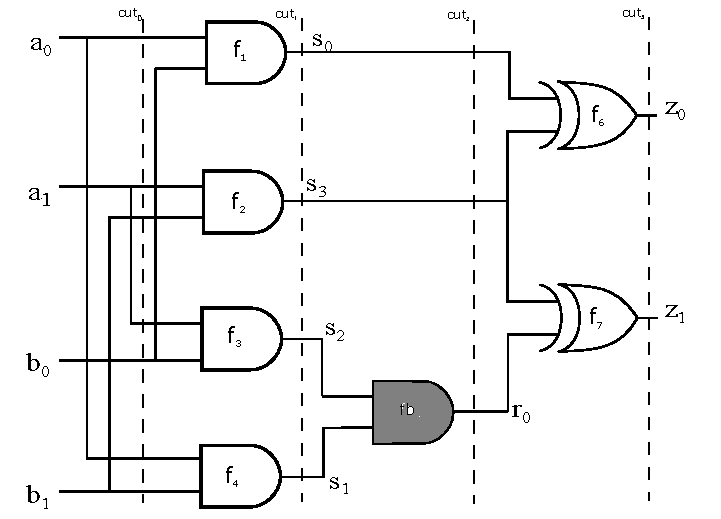
\includegraphics[scale = 0.75]{mas_b}
	\end{center}
	\vspace{-2ex}
	\caption{Buggy 2-bit mastrovito multiplier with redundancy}
	\label{mas_b}
	\vspace{-1ex}
\end{figure*}

\begin{Example}
Consider the buggy implementation of a 2-bit mastrovito multiplier as shown
in ~\autoref{mas_b}. The system is modeled over the ring
$R=\F_4[a_0,b_0,a_1,b_1,s_0,s_1,s_2,s_3,s_4,s_5,e_0,e_1,e_2,e_3,r_0,z_0,$
  $z_1,Z,A,B]$. 

The multiplier specification is given as $f: Z + A\cdot B$.

\subsection{Problem setup}
\begin{enumerate}
\item{Field construction: $\F_4 = \F_2[X]$ (mod $\mathcal{P}$); where $\mathcal{P} = X^2 + X + 1$ is the primitive polynomial used.}
\item{$Z = z_0 +\al z_1; A = a_0 +\al a_1; B = b_0 +\al b_1;$ are the word level polynomials, and $\al$ is the root of primitive polynomial s.t. $\mathcal{P}(\al)=0$.}
\end{enumerate}
Based on the circuit topology, RTTO$>$ with variable order:
$\{Z\}>\{A>B\}>\{z_0>z_1\}>\{r_0\}>\{e_0>e_1\}>\{e_2\}$ $>\{e_3\}>\{s_0>s_1>s_2>s_3>s_4>s_5\}>\{a_0>a_1>b_0>b_1\}$

Let $F$ be the set of all polynomials implementing the circuit which is given as:
% \begin{equation*}
% \begin{split}
% f_1:s_0 + a_0*b_0;  &  f_5:r_0 + s_1 + s_2; & f_8:A + a_0 + a_1*\al; \\
% f_2:s_3 + \mathcal{F}(a_1,b_1);  &  f_6:z_0 + s_0 + s_3; & f_9:B + b_0 + b_1*\al;\\
% f_3:s_2 + a_1*b_0;  &  f_7:z_1 + r_0 + s_3; & f_{10}:Z + z_0 + z_1*\al;\\
% f_4:s_1 + a_0*b_1;
% \end{split}
% \begin{equation}
{\small\begin{flalign*}
f_1:Z + z_0 +\al z_1;  &\quad f_9:e_2 + e_3 + s_4;   \\
f_2:A + a_0 +\al a_1;  &\quad \textcolor{red}{f_{10}:e_3 + b_0 + s_3;} \\
f_3:B + b_0 +\al b_1;  &\quad f_{11}:s_0 + a_0b_0; \\
f_4:z_0 + s_0 + e_0;	&\quad f_{12}:s_1 + a_1b_1; \\
f_5:z_1 + e_0 + r_0;	&\quad f_{13}:s_2 + a_1b_0; \\
f_6:r_0 + e_1 + s_5;	&\quad f_{14}:s_3 + a_0 + b_0 + a_0b_0; \\
f_7:e_0 + s_1e_2;       &\quad f_{15}:s_4 + b_0 + 1;\\
f_8:e_1 + s_2e_2;		&\quad f_{16}:s_5 + a_0b_1;
\end{flalign*}}

For the ease of explanation, we have taken a single gate bug as our fault model. As shown in the ~\autoref{mas_b},
the marked gate $f_{10}$ is the buggy XOR gate replacing the original AND gate.

Let $J_0 = \langle x_l^4 - x_l\rangle$ denote the ideal of vanishing
polynomials in $R$. Given the RTTO> order, we will have ideal of vanishing polynomials $J_0$ for primary inputs only.  
{\small\begin{flalign*}
f_{17}:a_0^2 + a_0; \\
f_{18}:a_1^2 + a_1; \\
f_{19}:b_0^2 + b_0; \\
f_{20}:b_1^2 + b_1; 
\end{flalign*}}%
\begin{small}

Then $F = \{f_1,\dots,f_{16}\}, J = \langle      F\rangle = \langle
f_1,\dots,f_{16}\rangle$
%J_0 = \langle f_{17},\dots,f_{20}\rangle$
\end{small}
% Due to RTTO$>$, the set of polynomials ($J+J_0$) is in itself a \Grobner basis.\\

\subsection{Verification}
For a correct implementation, the specification $f$ should be in $J + J_0$.
%vanishes on circuit implementation~(\autoref{lem:imt}):

% \begin{equation}
$f \in \langle f_1,f_2,f_3,\dots,f_{16}\rangle+J_0$

$f \xrightarrow[]{GB(J+J_0)}_{(\al+1)a_0a_1b_1b_0+(\al+1)a_0a_1b_1+(\al+1)a_1b_1b_0+(\al)a_1b_0}$

Since, the remainder is non zero, the circuit doesn't implement the specification and needs to be debugged.

\subsection{Remainder partition and cone pruning}
Given the elimination order under RTTO, the remainder will contain variables only from primary inputs.
We will group these monomials based on their coefficients and record all the group coefficients.

$r=(\al+1)a_0a_1b_1b_0+(\al+1)a_0a_1b_1+(\al+1)a_1b_1b_0+(\al)a_1b_0$

$r=\al*(a_0a_1b_1b_0+a_0a_1b_1+a_1b_1b_0+a_1b_0) + 1*(a_0a_1b_1b_0+a_0a_1b_1+a_1b_1b_0)$

$coeffs = \{\al,1\}$

Since the remainder was derived by reducing primary outputs, the the recorded coefficients represent the coefficients of outputs where the 
bug got propagated. By matching the recorded coefficients with the coefficients of outputs, we will derive the list of all affected outputs.

$coefficient(z_0) = 1$;
$coefficient(z_1) = \al$

Since we have both $\{1,\al\}$ in the coefficient record($coeffs$), all the outputs ($z_0,z_1$) are affected and their respective cones
need to be checked for rectification.

$affected\_outputs = \{z_0,z_1\}$

For a single output function, all the nets in the circuit are potential rectifiable nets since it has single coefficient. 
In case of multi-output, a single fix rectification might exist only at the intersection of all the buggy cones as the error propagation is affecting all the outputs marked by the remainder coefficients.

logical cones of each outputs are given as
$cone_{z_0}=(s_4,s_3,s_1,s_0,e_3,e_2,e_0,z_0)$

$cone_{z_1}=(s_5,s_4,s_3,s_2,s_1,e_3,e_2,e_1,e_0,r_0,z_1)$

$prune\_cone = cone_{z_0}\cap cone_{z_1} = \{s_4,s_3,s_2,s_1,e_3,e_2,e_0\}$

\subsection{Rectification check}
We will be checking for a single fix rectification within the pruned cone by sweeping the nets from primary input side in the topological order of the circuit.
This is to ensure that we try and find a rectification point as early as possible in the topology.
Given the highly irredundant nature of the finite field benchmarks, most of the circuits will allow a rectification fix 
early in the topology, if one exists. 

Based on the circuit topology, we will check for a single fix rectification existence at given nets in the order($\{s_4>s_3$ $>s_2>s_1>e_3>e_2>e_0\}$).
We will perform the rectification check in the topological order until we find a net which satisfies the single fix rectification condition or until we exhaust the potential 
rectifiable nets. In the former case we return the net where a single fix rectification exists, while in the latter case we exit the program indicating the absence of single fix rectification for the given bugs.

For checking the existence of rectification for the net under consideration, we will form two ideals ($J_L,J_H$) with the net polynomial modified as shown below.  

Since ($s_4$) is the first net to be checked for a fix, we will mark the polynomial $f_{15}$ which has leading term $s_4$ for modification.

$J_L = \langle f_1,f_2\dots f_{15}:s_4+1\dots f_{16}\rangle$

$J_H = \langle f_1,f_2\dots f_{15}:s_4\dots f_{16}\rangle$

By reducing spec using the above ideals we derive the remainders for the respective ideals.

$r_L = f \xrightarrow[]{J_L}_{(\al+1)a_0a_1b_1b_0+(\al+1)a_0a_1b_1}$

$r_H = f \xrightarrow[]{J_H}_{(\al+1)a_0a_1b_1b_0+(\al+1)a_0a_1b_1+(\al+1)a_1b_1+(\al)a_1b_0}$

From theorem~\ref{reference to rect check proof}-  

% $\overline{V(r_L)} \cap \overline{V(r_H)} = \emptyset$

% $V(r_L) \union V(r_H) = \Fq = V(J_0)$

% Since ideals and varieties are dual of each other, we can express union of varieties as product of ideals.

% $r_L*r_H = J_0$

% We compute the reduced GB of ideal product $((r_L*r_H) + J_0)$ and check if this ideal is equal to the ideal of vanishing polynomials.

$G_r = Grobner\_basis((r_L*r_H)+J_0)$

The computed $G_r$ for rectification check at net $s_4$ is given as:

$G_r[1]=b_0^2+b_0; G_r[2]=b_1^2+b_1;$

$G_r[3]=a_1^2+a_1;G_r[4]=a_0^2+a_0$

Since the computed product of ideals is equal to the ideal of vanishing polynomials, a single fix rectification exists at net $s_4$.

For the sake of comparison if a similar check was performed at net $s_1$, then the rectification check results would be as shown:

$J_L = \langle f_1,f_2\dots f_{12}:s_1+1\dots f_{16}\rangle$

$J_H = \langle f_1,f_2\dots f_{12}:s_14\dots f_{16}\rangle$

$r_L = f \xrightarrow[]{J_L}_{(\al+1)(a_0b_0+a_0+a_1b_1+b_0+1)+(\al)a_1b_0}$

$r_H = f \xrightarrow[]{J_H}_{(\al+1)a_1b_1+(\al)a_1b_0}$

$G_r = Grobner\_basis((r_L*r_H)+J_0)$

The computed $G_r$ for check at net $s_1$ is given as:

$G_r[1]=b_0^2+b_0; G_r[2]=b_1^2+b_1;$

$G_r[3]=a_1b_0; G_r[4]=a_1^2+a_1;$

$G_r[5]=a_0a_1b_1+(\al+1)a_0a_1b_0^2+a_0a_1b_0;$

$G_r[6]=a_0^2+a_0$

Since the computed product of ideals is not equal to the ideal of vanishing polynomials, a single fix rectification does not exist at net $s_1$.

\subsection{Correction function computation}
For the sake of simplicity, this example will show the correction function computation at net($e_3$).
To start with, we will mark the gate $f_{10}$ as the \textit{unknown
  component} in the design which is of the form $f_{10} = e_3 + P$,
where $P$ is the unknown function to be implemented by the gate. We
know that under RTTO $>$, the given set of circuit polynomials $F$
itself form a $GB$. Hence to compute $r$, we start reducing the 
specification polynomial $f$ using polynomials from $\langle J + J_0\rangle$.  

We will use the following notations for reduction: '[]' to represent quotient-$h_j$'s, '()' to represent divisor-$f_j$'s, and '\{\}' to represent the partial remainder of every reduction step-$fp_j$'s.

\begin{tiny}
% \begin{split}
$f\xrightarrow[]{f_{1}}[1](Z + z_0 +\al z_1)+\underbrace{{\scriptstyle \{AB+z_0+\al z_1\}}}_\text{$fp_1$}$

$fp_1\xrightarrow[]{f_2}[B](A+a_0+\al a_1)+\underbrace{{\scriptstyle \{Ba_0+\al Ba_1+z_0+\al z_1\}}}_\text{$fp_2$}$

$fp_2\xrightarrow[]{f_3}[a_0+\al a_1](B+b_0+\al b_1)+\underbrace{{\scriptstyle\{z_0+\al z_1+\al a_0b_1+a_0b_0+ (\al+1)a_1b_1 + \al a_1b_0\}}}_\text{$fp_3$}$

$fp_3\xrightarrow[]{f_4}[1](z_0+e_0+s_0)+\underbrace{{\scriptstyle\{\al z_1+e_0+s_0+\al a_0b_1+a_0b_0+(\al+1)a_1b_1+\al a_1b_0\}}}_\text{$fp_4$}$

$fp_4\xrightarrow[]{f_5}[\al](z_1+r_0+e_0)+\underbrace{{\scriptstyle\{\al z_1+e_0+s_0+\al a_0b_1+a_0b_0+(\al+1)a_1b_1+\al a_1b_0\}}}_\text{$fp_5$}$

$fp_5\xrightarrow[]{f_6}[\al](r_0+e_1+s_5)+\underbrace{{\scriptstyle\{(\al+1)e_0+\al e_1+s_0+\al s_5+\al a_0b_1+a_0b_0+(\al+1)a_1b_1+\al a_1b_0\}}}_\text{$fp_6$}$

$fp_6\xrightarrow[]{f_7}[\al+1](e_0+e_2*s_1)+\underbrace{{\scriptstyle\{\al e_1+(\al+1)e_2s_1+s_0+\al s_5+\al a_0b_1+a_0b_0+(\al+1)a_1b_1+\al a_1b_0\}}}_\text{$fp_7$}$

$fp_7\xrightarrow[]{f_8}[\al](e_1+e_2*s_2)+\underbrace{{\scriptstyle\{(\al+1)e_2s_1+\al e_2s_2 + s_0+\al s_5+\al a_0b_1+a_0b_0+(\al+1)a_1b_1+\al a_1b_0\}}}_\text{$fp_8$}$

$fp_8\xrightarrow[]{f_9}[(\al+1)s_1 + \al s_2](e_2+e_3+s_4)+\underbrace{{\scriptstyle\{(\al+1)e_3s_1+ \al e_3s_2 +s_0+(\al+1)s_1s_4+\al s_2s_4+\al s_5+\al a_0b_1+a_0b_0+(\al+1)a_1b_1+\al a_1b_0\}}}_\text{$fp_9$}$
\end{tiny}

\begin{small}

${\scriptstyle fp_9}\xrightarrow[]{{\scriptstyle lt(f_{10})}}[\underbrace{{\scriptstyle (\al+1)s_1+\al s_2}}_\text{$h_{10}$}]({\scriptstyle e_3})+$ 

$\underbrace{{\scriptstyle \{s_0+(\al+1)s_1s_4+\al s_2s_4+\al s_5+\al a_0b_1+a_0b_0+(\al+1)a_1b_1+\al a_1b_0\}}}_\text{$r$}$ 
\end{small}
% \end{split}

Reduction order for $f:$

$f\xrightarrow[]{f_{1}}\xrightarrow[]{f_2}\xrightarrow[]{f_3}\xrightarrow[]{f_4}\xrightarrow[]{f_5}\xrightarrow[]{f_6}\xrightarrow[]{f_7}\xrightarrow[]{f_8}\xrightarrow[]{f_9}\xrightarrow[]{lt(f_{10})}r$

% \begin{equation}
% \begin{split}
% h_4f_4+h_1f_1+h_2f_2+h_3f_3 = f+h_5f_5+h_6f_6+h_7f_7;\\
% h_4(d_0+P(e_1,c))+h_1f_1+h_2f_2+h_3f_3 = f+h_5f_5+h_6f_6+h_7f_7;\\
% h_4*d_0+h_4*P(e_1,c)+h_1f_1+h_2f_2+h_3f_3 = f+h_5f_5+h_6f_6+h_7f_7;\\
% h_4*P(e_1,c)+h_1f_1+h_2f_2+h_3f_3 = h_4*d_0+f+h_5f_5+h_6f_6+h_7f_7;\\
% h_4*P(e_1,c)+h_1f_1+h_2f_2+h_3f_3 = e_0*e_2+a*c+a+b*c+b+c;\\
% h_4*P(e_1,c)+h_1f_1+h_2f_2+h_3f_3 = e_0*e_2+a*c+a+b*c+b+c;
% \end{split}
% \end{equation}
Given: $r,h_{10},f_{11},f_{12},f_{13},f_{14},f_{15},f_{16},J_0$, the
problem can be formulated as an ideal membership test
using \eqref{eqn3} such that: 
\begin{center}
$r \in \langle h_{10},f_{11},f_{12},f_{13},f_{14},f_{15},f_{16}\rangle + \langle J_0\rangle$
\end{center}

The above ideal membership can be solved by expressing $r$ as a
linear combination of the ideal members (~\autoref{lem:imt}). 
\begin{small}
$r = Ph_{10} + h_{11}f_{11} + h_{12}f_{12}+h_{13}f_{13}+h_{14}f_{14}+h_{15}f_{15}+h_{16}f_{16}$ 
\end{small}

In our example, polynomial $r$ can be expressed as
%a linear combination ~(\autoref{lem:imt}) in given member ideal as
%follows:   

% \end{split}
% \end{equation}
\begin{small}
$r = [b_0]h_{10}+[1]f_{11}+[\al+1]f_{12}+[\al s_4 +\al b_0]f_{13}+[0]f_{14}+[(\al+1)s_1+\al a_1b_0]f_{15}+[\al]f_{16}+[0]f_{17}+[0]f_{18}+[0]f_{19}+[0]f_{20}$;
\end{small}

Thus computed $P=b_0$ is a solution to the \textit{unknown component}
$f_{10}$; i.e. $f_{10}: e_3 + b_0$.

Given a solution $P$, we can explore the solution space for 
the gate $f_i$ in terms of variables $x_j$ such that $x_i>x_j$ in the
variable order.
%This can be achieved by computing a quotient of
%ideals~(\autoref{def:quo}) and using different elimination
%ideals~(\autoref{def:elimideal}) with desired variables $x_j$ moved to
%the end of the variable order. 
In our example, $r$ can be written as:
% any linear combination of the ideals:

\begin{align*}
  \begin{split}
    r &= Ph_{10} + h_{11}f_{11} + h_{12}f_{12}+h_{13}f_{13}+h_{14}f_{14}\\
      &\quad +h_{15}f_{15}+h_{16}f_{16}+HJ_0
  \end{split}\\
  \begin{split}
  r & = P'h_{10} + h_{11}'f_{11} +  h_{12}'f_{12}+h_{13}'f_{13}+h_{14}'f_{14}\\
  &\quad +h_{15}'f_{15}+h_{16}'f_{16} + H'J_0
\end{split}
\end{align*}

Re-writing the above two equations:\\
\begin{align}
  \begin{split}
    (P-P')h_{10} &= (h_{11}-h_{11}')f_{11} + (h_{12}-h_{12}')f_{12}\\
    & \quad +\dots+(h_{16}-h_{16}')f_{16}+(H-H')J_0
  \end{split}\\
(P-P')h_{10} & \in  \langle f_{11},f_{12},\dots,f_{16},J_0\rangle\\
(P-P')       &\in     \langle f_{11},f_{12},\dots,f_{16},J_0\rangle:h_{10}\\
(P-P')       & \in  J_Q
\end{align}

The above expression for $J_Q$ represents the quotient of ideals
operation~(\autoref{def:quo}). We can pick any polynomial within
desired variable subset $x_j$ from the result of $J_Q$ and add it to the
computed solution $P$ to arrive at a new solution. 

Under the current $RTTO >$ variable order, the quotient of ideals
operation results in the following polynomials:\\ 
\begin{small}
$g[1]=b_1b_0+b_1+b_0+1\\
g[2]=(\al+1)b_1+(\al+1)*b_1*b_0+(\al+1)*b_0+(\al+1)\\
g[3]=a_1+1\\
g[4]=s_5+a_0b_1\\
g[5]=s_4+b_0+1\\
g[6]=s_3+a_0b_0+a_0+b_0\\
g[7]=s_2+b_0\\
g[8]=s_1+b_1\\
g[9]=s_0+a_0b_0$
\end{small}

Any $P+g[k]$, where $1<k<9$, will work as a solution for the
\textit{unknown component} $f_{10}$. 

Now assume that we know the immediate input variables of the
polynomial $f_{10}$ as $X_{im} = (b_0,s_3)$, we can compute a solution
in terms of these variables by using the elimination
ideal $J_Q \cap \Fq[b_0,s_3]$. The quotient
operation with the elimination ideal results in:\\ 
\begin{small}
$g[1]=s_3b_0 + b_0$
\end{small}

Since, there is only one $g$ from the operation, $P+g[1]=s_3b_0$ also
works as a solution for the \textit{unknown component}: $f_{10}: e_3 +
s_3b_0$. 

\end{Example}

%% \begin{Example}
%% Consider the 2-bit Mastrovito multiplier given in fig.~\ref{mas_c} with variables from ring $\R=\F_2[a_0,b_0$ $,a_1,b_1,s_0,s_1,s_2,s_3,r_0,z_0,z_1,Z,A,B]$. Let us assume $f_2$ to be the unknown gate in the design which is of the form $f_2 = s_3 + P$.\\%\mathcal{F}(a_1,b_1)$.\\


%% % For the given circuit, we define \textit{cuts} across the gates based on heuristics such as dependency and levelization\cite{maciej:2016:1}. A $cut$ is defined as a set of signals that separates primary inputs from primary outputs. The prominence of these cuts is to maintain a variable order across cuts . For example at each cut $cut_m$ from the figure(\ref{tianka_ckt_c}), the following variable set has to be maintained across reductions.
%% % \begin{equation}
%% % \begin{split}
%% % cut_0 = \{a,b,c\} &\quad cut_3= \{z_1,z_2\}\\
%% % cut_1 = \{e_0,e_1,c,e_2\}  &\quad cut_4 = \{z\} \\
%% % cut_2 = \{e_0,d_0,e_2\}
%% % \end{split}
%% % \end{equation}
%% The 2x2 Mastrovito multiplier with specification $f: Z + A\cdot B$, is constructed as follows:
%% % \begin{lalign*}
%% % \begin{split}
%% \begin{enumerate}
%%     \item{Field construction: $\F_4 = \F_2[X]$ (mod $\mathcal{P}$); where $\mathcal{P} = X^2 + X + 1$ is the primitive polynomial used.}
%%     \item{$Z = z_0 + z_1*\al; A = a_0 + a_1*\al; B = b_0 + b_1*\al;$ are the word level polynomials, and $\al$ is the root of primitive polynomial s.t. $\mathcal{P}(\al)=0$.}
%% \end{enumerate}
%% Based on the circuit topology, RTTO$>$ with variable order:
%% $\{Z\}>\{A>B\}>\{z_0>z_1\}>\{r_0>s_0>s_3\}>\{s_1>s_2$ $\}>\{a_0>a_1>b_0>b_1\}$\\ 
%% Let $F$ be the set of all polynomials implementing the circuit which are given as:
%% % \begin{equation*}
%% % \begin{split}
%% % f_1:s_0 + a_0*b_0;  &  f_5:r_0 + s_1 + s_2; & f_8:A + a_0 + a_1*\al; \\
%% % f_2:s_3 + \mathcal{F}(a_1,b_1);  &  f_6:z_0 + s_0 + s_3; & f_9:B + b_0 + b_1*\al;\\
%% % f_3:s_2 + a_1*b_0;  &  f_7:z_1 + r_0 + s_3; & f_{10}:Z + z_0 + z_1*\al;\\
%% % f_4:s_1 + a_0*b_1;
%% % \end{split}
%% % \begin{equation}
%% {\small\begin{flalign*}
%% f_1:s_0 + a_0*b_0;  &\quad  f_5:r_0 + s_1 + s_2; & f_8:A + a_0 + a_1*\al;\\
%% % f_2:s_3 + \mathcal{F}(a_1,b_1);  &\quad  f_6:z_0 + s_0 + s_3; & f_9:B + b_0 + b_1*\al;\\
%% f_2:s_3 + P;  &\quad  f_6:z_0 + s_0 + s_3; & f_9:B + b_0 + b_1*\al;\\
%% f_3:s_2 + a_1*b_0;  &\quad  f_7:z_1 + r_0 + s_3; & f_{10}:Z + z_0 + z_1*\al;\\
%% f_4:s_1 + a_0*b_1;
%% \end{flalign*}}%
%% We shall add the ideal of vanishing polynomials $J_0$ for primary inputs, outputs, and intermediate variables.  
%% {\small\begin{flalign*}
%% f_{11}:a_0^2 + a_0; &\quad f_{15}:s_0^2 + s_0;\quad f_{19}:r_0^2 + r_0;\quad f_{23}:A^4 + A;\\
%% f_{12}:a_1^2 + a_1; &\quad f_{16}:s_1^2 + s_1;\quad f_{20}:z_0^2 + z_0;\quad f_{24}:B^4 + B;\\
%% f_{13}:b_0^2 + b_0; &\quad f_{17}:s_2^2 + s_2;\quad f_{21}:z_1^2 + z_1;\\
%% f_{14}:b_1^2 + b_1; &\quad f_{18}:s_3^2 + s_3;\quad f_{22}:Z^4 + Z;
%% \end{flalign*}}%
%% \begin{small}
%% $F = \{f_1,\dots,f_{10}\}; J = \langle F\rangle = \langle f_1,\dots,f_{10}\rangle; J_0 = \langle f_{11},\dots,f_{24}\rangle$
%% \end{small}
%% % Due to RTTO$>$, the set of polynomials ($J+J_0$) is in itself a \Grobner basis.\\

%% For a correct implementation, specification $f$ vanishes on circuit implementation:
%% % \begin{equation}
%% $f \in \langle f_1,f_2,f_3,\dots,f_{10}\rangle+\langle f_{11},f_{12}$ $,\dots,f_{24}\rangle$,
%% % \end{equation}
%%  where tail of $f_2$ is unknown.
%% % h_4f_4 \in \langle f,f_1,f_2,f_3,f_5,f_6,f_7\rangle\\
%% % h_4f_4 = f+h_1f_1+h_2f_2+h_3f_3+h_5f_5+h_6f_6+h_7f_7

%% We know that under RTTO$>$, the given set of circuit polynomials in itself form a $GB$. Hence to compute $g$, we start reducing the specification polynomial $f$ using polynomials from the set $\langle J + J_0\rangle$. We will use the following notations for reduction: '[]' to represent quotient-$h_i$'s, '()' to represent divisor-$f_i$'s, and '\{\}' to represent the partial remainder of every reduction step-$fp_i$'s.

%% \begin{small}
%% % \begin{split}
%% $f\xrightarrow[]{f_{10}}[1](Z + z_0 + z_1*\al)+\{ A*B+z_0+\al*z_1\}\rightarrow fp_1$

%% $fp_1\xrightarrow[]{f_8}[B](A+a_0+\al*a_1)+\{B*a_0+\al*B*a_1+z_0+\al*z_1\}\rightarrow fp_2$

%% $fp_2\xrightarrow[]{f_9}[a_0+\al*a_1](B+b_0+\al*b_1)+\{z_0+\al*z_1+a_0*b_0+\al*a_0*b_1+\al*a_1*b_0+(\al+1)*a_1*b_1\}\rightarrow fp_3$

%% $fp_3\xrightarrow[]{f_6}[z_0+s_0+s_3](1)+\{\al*z_1+s_0+s_3+a_0*b_0+\al*a_0*b_1+\al*a_1*b_0+(\al+1)*a_1*b_1\}\rightarrow fp_4$

%% $fp_4\xrightarrow[]{f_7}[z_1+r_0+s_3](\al)+\{\al*r_0+s_0+(\al+1)*s_3+a_0*b_0+\al*a_0*b_1+\al*a_1*b_0+(\al+1)*a_1*b_1\}\rightarrow fp_5$

%% $fp_5\xrightarrow[]{f_5}[r_0+s_1+s_2](\al)+\{s_0+(\al+1)*s_3+\al*s_1+\al*s_2+a_0*b_0+\al*a_0*b_1+\al*a_1*b_0+(\al+1)*a_1*b_1\}\rightarrow fp_6$

%% $fp_6\xrightarrow[]{f_1}[s_0+a_0*b_0](1)+\{(\al+1)*s_3+\al*s_1+\al*s_2+\al*a_0*b_1+\al*a_1*b_0+(\al+1)*a_1*b_1\}\rightarrow fp_7$

%% % $fp_6\quad\xrightarrow[]{lt(f_2)}[s_3](\underbrace{x+1}_\text{$h_2$})+\{\underbrace{(x)*s_1+(x)*s_2+(x)*a_0*b_1+(x)*a_1*b_0+(x+1)*a_1*b_1}_\text{$g$}\}$
%% ${\scriptstyle fp_7}\xrightarrow[]{{\scriptstyle lt(f_2)}}[{\scriptstyle s_3}](\underbrace{{\scriptstyle \al+1}}_\text{$h_2$})+\{\underbrace{{\scriptstyle\al s_1+\al s_2+\al a_0b_1+\al a_1b_0+(\al+1)a_1b_1}}_\text{$g$}\}$


%% % \end{split}
%% \end{small}
%% Reduction order for $f:$
%% $f\xrightarrow[]{f_{10}}\xrightarrow[]{f_8}\xrightarrow[]{f_9}\xrightarrow[]{f_6}\xrightarrow[]{f_7}\xrightarrow[]{f_5}\xrightarrow[]{f_1}\xrightarrow[]{lt(f_2)}g$

%% % \begin{equation}
%% % \begin{split}
%% % h_4f_4+h_1f_1+h_2f_2+h_3f_3 = f+h_5f_5+h_6f_6+h_7f_7;\\
%% % h_4(d_0+P(e_1,c))+h_1f_1+h_2f_2+h_3f_3 = f+h_5f_5+h_6f_6+h_7f_7;\\
%% % h_4*d_0+h_4*P(e_1,c)+h_1f_1+h_2f_2+h_3f_3 = f+h_5f_5+h_6f_6+h_7f_7;\\
%% % h_4*P(e_1,c)+h_1f_1+h_2f_2+h_3f_3 = h_4*d_0+f+h_5f_5+h_6f_6+h_7f_7;\\
%% % h_4*P(e_1,c)+h_1f_1+h_2f_2+h_3f_3 = e_0*e_2+a*c+a+b*c+b+c;\\
%% % h_4*P(e_1,c)+h_1f_1+h_2f_2+h_3f_3 = e_0*e_2+a*c+a+b*c+b+c;
%% % \end{split}
%% % \end{equation}
%% Since, we know $g,h_2,f_3,f_4,J_0$, we can formulate it as ideal membership testing problem using~\eqref{member}:
%% \begin{center}
%% $g \in \langle h_2,f_3,f_4\rangle + \langle J_0\rangle$
%% \end{center}

%% This ideal membership test can be done using $lift$ procedure in SINGULAR~\cite{DGPS_410}. The procedure takes polynomial $f$, and ideal $J$ in row matrix form($[J+J_0]$) as inputs, and returns a column matrix $[U]$ as output such that:
%% \begin{small}
%% $f = [U]\cdot [J+J_0]$
%% \end{small}

%% % \begin{equation}
%% % \begin{split}
%% \begin{small}
%% $g = \begin{bmatrix} h_2^{'} & h_3^{'} & \dots & H \end{bmatrix} \cdot 
%%     \begin{bmatrix} h_2 \\ f_3 \\ \vdots \\ x_n^2 + x_n \end{bmatrix}$
%% \end{small}

%% The matrix output can be written in a linear combination as follows: 
%% % \end{split}
%% % \end{equation}
%% \begin{small}
%% $\al*s_1+\al*s_2+\al*a_0*b_1+\al*a_1*b_0+(\al+1)*a_1*b_1 = [\al*s_1+\al*s_2+\al*a_0*b_1+\al*a_1*b_0+(\al+1)*a_1*b_1](\al+1) + [0](s_2 + a_1*b_0) + [0](s_1 + a_0*b_1) + \dots + [0](x_n^2 + x_n)$;
%% \end{small}

%% The $lift$ procedure uses $GB$ to compute the linear combination. Since the generator set has a constant polynomial($\al+1$), the procedure considers it as constant one during membership computation. Hence the output in this case will be a 1x1 matrix with $g$ itself projected as the solution. To normalize the ignored constant, we need to divide(multiply the inverse) the solution $g$ by the constant$(\al+1)$ and reduce it with polynomials \{$f_3,f_4$\} in order to arrive at a implementable solution.

%% \begin{small}
%% $(\al+1)^{-1} = \al$

%% $h_2^{''} = \al*h_2^{'} = \al*(\al*s_1+\al*s_2+\al*a_0*b_1+\al*a_1*b_0+(\al+1)*a_1*b_1)$

%% $h_2^{''} = (\al+1)*s_1+(\al+1)*s_2+(\al+1)*a_0*b_1+(\al+1)*a_1*b_0+ a_1*b_1$

%% $h_2^{''}\xrightarrow[]{f_{3}}\xrightarrow[]{f_4}\underbrace{a_1*b_1}_\text{P}$
%% \end{small}

%% This computed $P$ is a valid solution and can be used as tail of $f_2$. If the resulting $P$ were not a solution in immediate support variables of $s_3$($a_1,b_1$), we could have arrived at this desired solution by devising a new term order. The new term order will have variables $(s_3,a_1,b_1)$ moved to the end on the variable order. We could then compute a $GB$ using the modified term order with the intermediate solution $P$ added as tail of $f_2$. This $GB$ will have one and only one polynomial which is of the form $s_3 + \mathcal{F}(a_1,b_1)$, where $\mathcal{F}$ is the function implemented by the gate for these variables.\\
%% Modified term order $\{Z\}>\{A>B\}>\{z_0>z_1\}>\{r_0>s_0\}>\{s_1>s_2$ $\}>\{a_0>b_0>s_3>a_1>b_1\}$.\\
%% To illustrate the computation of multiple solutions, let's take the current solution $a_1*b_1$ as our $P$. With RTTO$>$ as our term order, from~\eqref{quotcomp}:

%% $a_1*b_1 - P^{'} \in \{f_3,f_4,x_l^q-x_l\}:h_2$;\\
%% The result from quotient of ideal operation is given as:
%% {\small\begin{flalign*}
%% f_3:s_2 + a_1*b_0;  f_{13}:b_0^2 + b_0; f_{23}:A^4 + A;\\
%% f_4:s_1 + a_0*b_1;  f_{14}:b_1^2 + b_1; f_{24}:B^4 + B; \\
%% f_{11}:a_0^2 + a_0; f_{16}:s_1^2 + s_1; \\
%% f_{12}:a_1^2 + a_1; f_{17}:s_2^2 + s_2;
%% \end{flalign*}}%
%% Any polynomial from the above list when added in tail of $f_2$ along with $P$ satisfies the solution set for the given unknown component.
%% \end{Example}

% \subsection{Circuit implementation as reference}
% Consider a circuit implementation $C$, modeled as polynomials $F = \{f_1,\dots,f_s\}\in \mathbb{F}_q[in_j,x_1,\dots, x_n]$, with $J_1=\langle F \rangle$, $in_j$ as the set of all primary inputs, and $x_n$ as the word level output. Let us assume $f_i:1\le i \le s$ to be the unknown component which is of the special form:
% \begin{gather*} 
% f_i = x_i + P
% \end{gather*}

% Let us consider a different circuit $C_1$ as the golden specification which implements the same function as $C$. The reference circuit is modeled as polynomials $D = \{d_1,\dots d_r\}\in \mathbb{F}_q[in_j,y_1,\dots, y_m]$, with $J_2=\langle D \rangle$, $in_j$ as the set of all primary inputs, and $y_m$ as the word level output.

% To formulate the problem, we will derive a new circuit structure using the above two implementations ($C,C_1$). Primary input set $in_j$ will be used as the common set of inputs for both the circuits. A new specification polynomial $f$ is derived using the word level outputs as:
% \begin{gather}
% f_{spec} : (x_n-y_m)
% \end{gather}

% Now, for a correct implementation, specification $f$ should vanish on the variety of ideal generated by the circuit polynomials i.e., $f$ will be in the ideal generated by the circuit:

% $f \in J_1 + J_2 + J_0$: where $J_0$ is the set of all vanishing polynomials from circuits $C$ and $C_1$.

% {\small $f \in \langle f_1,\dots,f_s\rangle + \langle d_1,\dots,d_r\rangle + \langle x_l^q-x_l\rangle + \langle y_u^q-y_u\rangle$; $1\le l \le n,1\le u \le m$}

% The problem formulation is now exactly same as~\eqref{eqn1} with $f_i$ from circuit $C$ as the unknown gate. Now, we will follow the same procedure as in the first notion to realize the function of the unknown component. Once a solution has been computed, we can verify the circuit using principles from weak $\it{Nullstellensatz}$ by checking if $GB(J_1+J_2+J_0)=\{1\}$.

% \begin{algorithm}
% \caption{Resolve the unknown component for a given circuit}
% \label{algo:unknownComponent}
% \begin{algorithmic}[1]

% \Procedure{$multi\_variate\_division$}{$F,f$}

% \Procedure{$forward\_lifting$}{}

% \EndProcedure
% \end{algorithmic}
% \end{algorithm}

% Thus, $P(u_1)=P(e_1,c)=c$, which can implemented as a simple AND gate with $c$ as both inputs. 

% \begin{figure}[ht]
% 	\begin{center}
% 	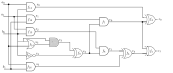
\includegraphics[scale = 0.40]{mas_c}
% 	\end{center}
% 	\vspace{-1ex}
% 	\caption{correct implementation mastrovito}
% 	\label{mas_c}
% 	\vspace{-1ex}
% \end{figure}

% \begin{figure}[ht]
% 	\begin{center}
% 	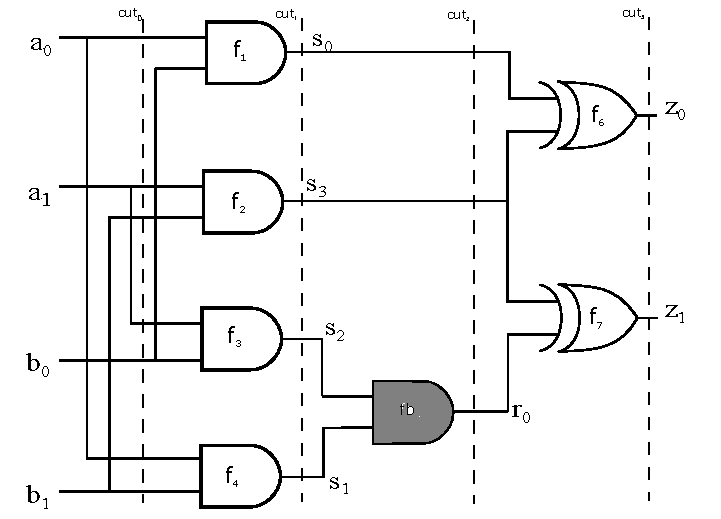
\includegraphics[scale = 0.40]{mas_b}
% 	\end{center}
% 	\vspace{-4ex}
% 	\caption{buggy implementation mastrovito}
% 	\label{mas_b}
% 	\vspace{-2ex}
% \end{figure}
